% Guidelines -> http://en.wikibooks.org/wiki/LaTeX/General_Guidelines
\documentclass[10pt,a4paper,landscape,twocolumn,twoside]{article}
\usepackage[english]{babel}
\usepackage[utf8]{inputenc}
\usepackage{graphicx}
\usepackage{anysize}
\usepackage{amsmath}
\usepackage{amssymb}
\usepackage{csquotes}
\usepackage[usenames,dvipsnames]{xcolor}
\usepackage{listings}
\usepackage{enumerate}
\usepackage{hyperref}
\usepackage{pdfpages}
\usepackage{titlesec}
\usepackage{makeidx}
\usepackage[columns=3]{idxlayout}

\newcommand{\BigO}[1]{\ensuremath{\operatorname{O}\bigl(#1\bigr)}}

\makeindex

\marginsize{1.5cm}{1.5cm}{0.8cm}{1cm} % control the margins {left}{right}{top}{bottom}.
\definecolor{gray99}{gray}{.99}

\lstset{
	language=C++,
	numbers=left,
	backgroundcolor=\color{gray99},
	tabsize=2,
	frame=single,
	keywordstyle=\ttfamily\bfseries\color{RoyalBlue},
	commentstyle=\ttfamily\color{ForestGreen},
	stringstyle=\ttfamily\color{Gray},
	breaklines=true,
	showstringspaces=false,
	basicstyle=\small\ttfamily,
	emph={label},
	xleftmargin=17pt,
	framexleftmargin=0pt,
	framexrightmargin=5pt,
	framexbottommargin=4pt,
}

\providecommand{\keywords}[1]{\textbf{\textit{Keywords---}} #1}

\titleformat{\section}
  {\normalfont\Large\bfseries}{\thesection}{1em}{}[{\titlerule[0.8pt]}]
\titleformat{\subsection}
  {\normalfont\bfseries}{\thesubsection}{1em}{}[{\titlerule[0.5pt]}]

\title{Algorithms Lab.}
\author{Álvaro Marco\\
		\texttt{amarco@inf.ethz.ch}
}
\date{\today}

\begin{document}

\maketitle

\tableofcontents

\section{Basic}
Include the line:
\begin{displayquote}
	\texttt{std::ios\_base::sync\_with\_stdio(false);}
\end{displayquote}
at the beginning of each program.

To print doubles specifying the precision use \texttt{setprecision}, e.g.:
\begin{displayquote}
	\texttt{cout << setprecision(7) << sum << endl;}
\end{displayquote}

For CGAL programs, add:
\begin{displayquote}
	\texttt{set(CMAKE\_CXX\_FLAGS ``\${CMAKE\_CXX\_FLAGS} -std=c++11'')}
\end{displayquote}
somewhere in the \texttt{CMakeLists.txt} file.

Whenever sets are needed consider \url{https://judge.inf.ethz.ch/doc/boost/libs/disjoint_sets/disjoint_sets.html}.

Figure~\ref{fig:neighbors} shows how the triangulation datastructure works with faces in CGAL. Check slides 19 and 20 in \url{https://judge.inf.ethz.ch/doc/course/cgal_proximity.pdf} for further information.

\begin{figure}[!ht]
\label{fig:neighbors}
	\centering
	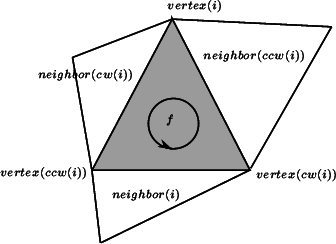
\includegraphics[width=0.25\textwidth]{img/neighbors.png}
	\caption{Vertices and neighbor faces in a CGAL triangulation.}
\end{figure}

	\subsection{Theory}
	\label{sub:Theory}
		\begin{itemize}
			\item A double can store integers until $2^{53}$
			\item Minimum independent set: maximum number of vertices s.t. there is no edge between the vertices (NP-COMPLETE! however OK for bipartite graph)
			\item Maximum vertex cover: Minimum number of vertices s.t. all the edges of the graph are included. Complementary to Minimum independent set (NP-COMPLETE! however OK for bipartite graph)
			\item König's theorem: In bipartite graphs, the size of a minimum vertex cover equals the size of a maximum matching. $|MIS| = n - |MVC|$
			\item $a \leq b \equiv -a \geq -b$
			\item $\max(f(x)) = -\min(-f(x))$
		\end{itemize}

\section{Complexities}
	\subsection{Boost Graph Library}
		\begin{itemize}
			\item Connected components (\texttt{connected\_components}): $ \BigO{V + E} $
			\item Cycle cancelling (\texttt{cycle\_canceling}): $ \BigO{C \cdot (EV)} $ where C is the cost of the initial flow
			\item Dijkstra (\texttt{dijkstra\_shortest\_paths}): $ \BigO{V \log V + E} $
			\item Kruskal MST (\texttt{kruskal\_minimum\_spanning\_tree}): $ \BigO{E \log E} $
			\item Prim MST (\texttt{prim\_minimum\_spanning\_tree}): $ \BigO{E \log V} $
			\item Push relabel max flow (\texttt{push\_relabel\_max\_flow}): $ \BigO{V^{3}} $
			\item Strong components (\texttt{strong\_components}): $ \BigO{V + E} $
			\item Succesive shortest path nonneg\ldots (\texttt{successive\_shortest\_path\_nonnegative\_weights}): $ \BigO{|f|(E + V \log V)} $
		\end{itemize}

	\subsubsection{CGAL}
	\label{subs:CGAL}
		Use Kernels in the following order of preference:
		\begin{enumerate}
			\item \texttt{CGAL::Exact\_predicates\_inexact\_constructions\_kernel} (constructions use \texttt{double})
			\item \texttt{CGAL::Exact\_predicates\_exact\_constructions\_kernel} (constructions use an exact number type)
			\item \texttt{CGAL::Exact\_predicates\_exact\_constructions\_kernel\_with\_sqrt}
		\end{enumerate}

		\textbf{Try to avoid constructions.}

\newpage
\section{Problems}
%
% 	\subsection{Introduction}

		% \subsubsection{Build the sum}
		% \begin{keywords}Floating point formatting\end{keywords}
		% \index{Floating point formatting}
		% %\includepdf[pages=-]{../week1/build_sum/buildthesum.pdf}
		% \lstinputlisting{../week1/build_sum/build_sum.cpp}

		% \subsubsection{Dominoes}
		% %\includepdf[pages=-]{../week1/dominoes/dominoes.pdf}
		% \lstinputlisting{../week1/dominoes/dominoes.cpp}

		% \subsubsection{Even pairs}
		% %\includepdf[pages=-]{../week1/even_pairs/even_pairs.pdf}
		% \lstinputlisting{../week1/even_pairs/even_pairs.cpp}

		% \subsubsection{False coin}
		% %\includepdf[pages=-]{../week1/false_coin/false_coin.pdf}
		% \lstinputlisting{../week1/false_coin/false_coin.cpp}

		% \subsubsection{Shelves}
		% Check \url{https://judge.inf.ethz.ch/doc/course/bfs_dfs_greedy.pdf}
		% %\includepdf[pages=-]{../week1/shelves/shelves.pdf}
		% \lstinputlisting{../week1/shelves/shelves.cpp}

	% \newpage
	\subsection{Greedy \& BFS/DFS}

		\subsubsection{Aliens}
		\begin{keywords}Custom sort\end{keywords}
		\index{Custom sort}
		%\includepdf[pages=-]{../week2/aliens/aliens.pdf}
		\lstinputlisting{../week2/aliens/aliens.cpp}

		\subsubsection{Boats}
		\begin{keywords}Greedy, Intervals\end{keywords}
		\index{Greedy}
		\index{Intervals}
		%\includepdf[pages=-]{../week2/boats/boats.pdf}
		\lstinputlisting{../week2/boats/boats.cpp}

		\subsubsection{Next path}
		\begin{keywords}BFS\end{keywords}
		\index{BFS}
		%\includepdf[pages=-]{../week2/nextpath/nextpath.pdf}
		\lstinputlisting{../week2/nextpath/nextpath.cpp}

		\subsubsection{Race tracks}
		\begin{keywords}BFS\end{keywords}
		\index{BFS}
		%\includepdf[pages=-]{../week2/racetracks/racetracks.pdf}
		\lstinputlisting{../week2/racetracks/racetracks.cpp}

		\subsubsection{Snippets}
		\begin{keywords}priority\_queue\end{keywords}
		\index{priority\_queue}
		%\includepdf[pages=-]{../week3/snippets/snippets.pdf}
		\lstinputlisting{../week3/snippets/snippets.cpp}

	\newpage
	\subsection{CGAL basic}

		\subsubsection{Antenna}
		\begin{keywords}ceil\_to\_double, Min\_circle\_2\end{keywords}
		\index{ceil\_to\_double}
		\index{Min\_circle\_2}
		%\includepdf[pages=-]{../week3/antenna/antenna.pdf}
		\lstinputlisting{../week3/antenna/antenna.cpp}

		\subsubsection{Almost antenna}
		\begin{keywords}Min\_circle\_2\end{keywords}
		\index{Min\_circle\_2}
		%\includepdf[pages=-]{../week3/almost_antenna/almost_antenna.pdf}
		\lstinputlisting{../week3/almost_antenna/almost_antenna.cpp}

		\subsubsection{Hiking maps}
		\begin{keywords}all\_of, left\_turn\end{keywords}
		\index{all\_of}
		\index{left\_turn}
		%\includepdf[pages=-]{../week4/hiking_maps/hiking_maps.pdf}
		\lstinputlisting{../week4/hiking_maps/hiking_maps.cpp}

		\subsubsection{Hit}
		\begin{keywords}do\_intersect, Ray\_2, Segment\_2\end{keywords}
		\index{do\_intersect}
		\index{Ray\_2}
		\index{Segment\_2}
		%\includepdf[pages=-]{../week3/hit/hit.pdf}
		\lstinputlisting{../week3/hit/hit.cpp}

		\subsubsection{First hit}
		\begin{keywords}floor\_to\_double, intersection\end{keywords}
		\index{floor\_to\_double}
		\index{intersection}
		%\includepdf[pages=-]{../week3/firsthit/firsthit.pdf}
		\lstinputlisting{../week3/firsthit/firsthit.cpp}

	\newpage
	\subsection{Graphs: Dijkstra \& MST}

		\subsubsection{Ant challenge}
		\begin{keywords}Dijkstra, Kruskal\end{keywords}
		\index{Dijkstra}
		\index{Kruskal MST}
		%\includepdf[pages=-]{../week4/ant_challenge/ant_challenge.pdf}
		\lstinputlisting{../week4/ant_challenge/ant_challenge.cpp}

		\subsubsection{First steps BGL}
		\begin{keywords}Dijkstra, Kruskal\end{keywords}
		\index{Dijkstra}
		\index{Kruskal MST}
		%\includepdf[pages=-]{../week4/first_steps_bgl/first_steps_bgl.pdf}
		\lstinputlisting{../week4/first_steps_bgl/first_steps_bgl.cpp}

		\subsubsection{Important bridges}
		\begin{keywords}Custom sort, Kruskal\end{keywords}
		\index{Custom sort}
		\index{Kruskal MST}
		%\includepdf[pages=-]{../week4/important_bridges/important_bridges.pdf}
		\lstinputlisting{../week4/important_bridges/important_bridges.cpp}

		\subsubsection{Return of the Jedi}
		\begin{keywords}Kruskal, Second MST\end{keywords}
		\index{Kruskal MST}
		\index{Second MST}

		Check \url{https://judge.inf.ethz.ch/doc/course/return_of_the_jedi.pdf}
		%\includepdf[pages=-]{../week10/return_of_the_jedi/return_of_the_jedi.pdf}
		\lstinputlisting{../week10/return_of_the_jedi/return_of_the_jedi.cpp}

		\subsubsection{Tracking}
		\begin{keywords}Dijkstra\end{keywords}
		\index{Dijkstra}
		%\includepdf[pages=-]{../week5/tracking/tracking.pdf}
		\lstinputlisting{../week5/tracking/tracking.cpp}

	\newpage
	\subsection{Dynamic programming}

		\subsubsection{Bonus level}
		\label{subs:Bonus level DP}
		\begin{keywords}\end{keywords}
		ATTENTION! this solution gives only 80 points! (100 probably replacing the \texttt{map} by a \texttt{vector}) check \ref{subs:Bonus level} for 100 points
		%\index{}
		%\includepdf[pages=-]{../week11/bonus_level/bonus_level.pdf}
		\lstinputlisting{../week11/bonus_level/bonus_level_dp_80.cpp}

		\subsubsection{Burning coins from two sides}
		\label{subs:Burning coins from two sides}
		\begin{keywords}Minimax\end{keywords}
		\index{Minimax}
		%\includepdf[pages=-]{../week10/burning_coins/burning_coins.pdf}
		\lstinputlisting{../week10/burning_coins/burning_coins.cpp}

		\subsubsection{DHL}
		%\includepdf[pages=-]{../week5/dhl/dhl.pdf}
		\lstinputlisting{../week5/dhl/dhl.cpp}

		\subsubsection{Poker chips}
		Unfortunately only 30 points :(
		%\includepdf[pages=-]{../week5/poker_chips/poker_chips.pdf}
		\lstinputlisting{../week5/poker_chips/poker_chips_30.cpp}

		\subsubsection{The great game}
		\begin{keywords}Minimax, max\_element, min\_element\end{keywords}
		\index{Minimax}
		\index{max\_element}
		\index{min\_element}
		%\includepdf[pages=-]{../week6/the_great_game/the_great_game.pdf}
		\lstinputlisting{../week6/the_great_game/the_great_game.cpp}

	\newpage
	\subsection{Network flows}
	\label{sub:Network flows}

		\subsubsection{Coin tossing}
		%\begin{keywords}minimax\end{keywords}
		%\index{minimax}
		%\includepdf[pages=-]{../week6/coin_tossing/coin_tossing.pdf}
		\lstinputlisting{../week6/coin_tossing/coin_tossing.cpp}

		\subsubsection{Kingdom defence}
		\begin{keywords}Minimum flow per edge\end{keywords}
		\index{Minimum flow per edge}
		%\includepdf[pages=-]{../week6/kingdom_defence/kingdom_defence.pdf}
		\lstinputlisting{../week6/kingdom_defence/kingdom_defence.cpp}

		\subsubsection{Shopping trip}
		\begin{keywords}Edge disjoint paths\end{keywords}
		\index{Edge disjoint paths}
		%\includepdf[pages=-]{../week6/shopping_trip/shopping_trip.pdf}
		\lstinputlisting{../week6/shopping_trip/shopping_trip.cpp}

		\subsubsection{Tetris}
		\label{subs:tetris}
		\begin{keywords}Vertex capacities\end{keywords}
		\index{Vertex capacities}
		%\includepdf[pages=-]{../week7/tetris/tetris.pdf}
		\lstinputlisting{../week13/tetris/tetris.cpp}

		\subsubsection{The phantom menace}
		\label{subs:menace}
		\begin{keywords}Vertex capacities\end{keywords}
		\index{Vertex capacities}
		%\includepdf[pages=-]{../week7/the_phantom_menace/the_phantom_menace.pdf}
		\lstinputlisting{../week7/the_phantom_menace/the_phantom_menace.cpp}

	\newpage
	\subsection{Linear programming}
	\label{sub:Linear programming}

		\subsubsection{Diet}
		\label{subs:Diet}
		\begin{keywords}floor\_to\_double\end{keywords}
		\index{floor\_to\_double}
		%\includepdf[pages=-]{../week7/diet/diet.pdf}
		\lstinputlisting{../week7/diet/diet.cpp}

		\subsubsection{Inball}
		\label{subs:Inball}
		\begin{keywords}\end{keywords}
		%\index{}
		%\includepdf[pages=-]{../week7/inball/inball.pdf}
		\lstinputlisting{../week7/inball/inball.cpp}

		\subsubsection{Maximize it}
		\label{subs:Maximize}
		\begin{keywords}Quadratic programming\end{keywords}
		\index{Quadratic programming}
		%\includepdf[pages=-]{../week7/maximize_it/maximize_it.pdf}
		\lstinputlisting{../week7/maximize_it/maximize_it.cpp}

		\subsubsection{Portfolios}
		\label{subs:Portfolios}
		\begin{keywords}Quadratic programming\end{keywords}
		\index{Quadratic programming}
		%\includepdf[pages=-]{../week7/portfolios/portfolios.pdf}
		\lstinputlisting{../week7/portfolios/portfolios.cpp}

		\subsubsection{Portfolios revisited}
		\label{subs:Portfolios revisited}
		\begin{keywords}Binary search, Quadratic programming\end{keywords}
		\index{Binary search}
		\index{Quadratic programming}
		%\includepdf[pages=-]{../week11/portfolios_revisited/portfolios_revisited.pdf}
		\lstinputlisting{../week11/portfolios_revisited/portfolios_revisited.cpp}

		% \subsubsection{Radiation}
		% \label{subs:Radiation}
		% \begin{keywords}Binary search, Strictly greater inequality\end{keywords}
		% \index{Binary search}
		% \index{Strictly greater inequality}
    %
		% Linear search with correct Linear program. After this version, binary search Linear program (100 pt) but the stictly greater operation not implemented properly.
		% %\includepdf[pages=-]{../week12/radiation/radiation.pdf}
		% \lstinputlisting{../week12/radiation/radiation_linear.cpp}
		% \lstinputlisting{../week12/radiation/radiation.cpp}

	\newpage
	\subsection{CGAL proximity structures}
	\label{sub:CGAL proximity structures}

		\subsubsection{Bistro}
		\label{subs:Bistro}
		\begin{keywords}Triangulation, nearest\_vertex\end{keywords}
		\index{Triangulation}
		\index{nearest\_vertex}
		Distance to closest point in triangulation.
		%\includepdf[pages=-]{../week8/bistro/bistro.pdf}
		\lstinputlisting{../week8/bistro/bistro.cpp}

		\subsubsection{Germs}
		\label{subs:Germs}
		\begin{keywords}\end{keywords}
		%\index{}
		%\includepdf[pages=-]{../week8/germs/germs.pdf}
		\lstinputlisting{../week8/germs/germs.cpp}

		\subsubsection{Graypes}
		\label{subs:Graypes}
		\begin{keywords}\end{keywords}
		%\index{}
		Minimum distance between all possible pairs of elements in a triangulation.
		%\includepdf[pages=-]{../week8/graypes/graypes.pdf}
		\lstinputlisting{../week8/graypes/graypes.cpp}

		\subsubsection{H1N1}
		\label{subs:H1N1}
		\begin{keywords}Motion planning, Triangulation DFS\end{keywords}
		\index{Motion planning}
		\index{Triangulation DFS}
		%\includepdf[pages=-]{../week8/h1n1/h1n1.pdf}
		\lstinputlisting{../week8/h1n1/h1n1.cpp}

		\subsubsection{Light the stage}
		\label{subs:Light the stage}
		\begin{keywords}Triangulation\end{keywords}
		\index{Triangulation}
		%\includepdf[pages=-]{../week10/light_the_stage/light_the_stage.pdf}
		\lstinputlisting{../week10/light_the_stage/light_the_stage.cpp}

	\newpage
	\subsection{Minimum cut, Bipartite matching}
	\label{sub:Minimum cut, Bipartite matching}

		\subsubsection{Algocoon}
		\label{subs:Algocoon}
		\begin{keywords}Minimum cut\end{keywords}
		\index{Minimum cut}

		Check \url{https://judge.inf.ethz.ch/doc/course/algocoon_group.pdf}
		%\includepdf[pages=-]{../week9/algocoon/algocoon.pdf}
		\lstinputlisting{../week9/algocoon/algocoon.cpp}

		\subsubsection{Knights}
		\label{subs:Knights}
		\begin{keywords}Minimum vertex cover\end{keywords}
		\index{Minimum vertex cover}
		%\includepdf[pages=-]{../week11/knights/knights.pdf}
		\lstinputlisting{../week11/knights/knights.cpp}

		\subsubsection{New hope}
		\label{subs:New hope}
		\begin{keywords}Bipartite graph, is\_bipartite, Minimum vertex cover\end{keywords}
		\index{Bipartite graph}
		\index{is\_bipartite}
		\index{Minimum vertex cover}

		50 points. It only works when there is a unique stormtrooper per command center.
		%\includepdf[pages=-]{../week13/new_hope/new_hope.pdf}
		\lstinputlisting{../week13/new_hope/new_hope_50.cpp}

		\subsubsection{Satellites}
		\label{subs:Satellites}
		\begin{keywords}Minimum vertex cover, No-source no-sink\end{keywords}
		\index{Minimum vertex cover}
		\index{No-source no-sink}
		%\includepdf[pages=-]{../week9/satellites/satellites.pdf}
		\lstinputlisting{../week9/satellites/satellites.cpp}

	\newpage
	\subsection{Min cost max flow}
	\label{sub:Min cost max flow}

		\subsubsection{Bonus level}
		\label{subs:Bonus level}
		\begin{keywords}\end{keywords}
		%\index{}

		Check \url{https://judge.inf.ethz.ch/doc/course/solution_bonus_level.pdf}
		%\includepdf[pages=-]{../week11/bonus_level/bonus_level.pdf}
		\lstinputlisting{../week11/bonus_level/bonus_level.cpp}

		\subsubsection{Canteen}
		\label{subs:Canteen}
		\begin{keywords}\end{keywords}

		Check \url{https://judge.inf.ethz.ch/doc/course/canteen.pdf}
		%\includepdf[pages=-]{../week9/canteen/canteen.pdf}
		\lstinputlisting{../week9/canteen/canteen.cpp}

		\subsubsection{Carsharing}
		\label{subs:Carsharing}
		\begin{keywords}equal\_range\end{keywords}
		\index{equal\_range}

		Check \url{https://judge.inf.ethz.ch/doc/course/carsharing.pdf}
		%\includepdf[pages=-]{../week13/carsharing/carsharing.pdf}
		\lstinputlisting{../week13/carsharing/carsharing.cpp}

		\subsubsection{Real estate market}
		\label{subs:Real estate market}
		\begin{keywords}Integer programming\end{keywords}
		\index{Integer programming}

		Check \url{https://judge.inf.ethz.ch/doc/course/real_estate_handout.pdf}
		%\includepdf[pages=-]{../week9/real_estate_market/real_estate_market.pdf}
		\lstinputlisting{../week9/real_estate_market/real_estate_market.cpp}

	\newpage
	\subsection{Miscellaneous}

		\subsubsection{Buddy selection}
		\begin{keywords}Max cardinality matching, Set intersection\end{keywords}
		\index{Max cardinality matching}
		\index{Set intertsection}
		%\includepdf[pages=-]{../week4/buddy_selection/buddy_selection.pdf}
		\lstinputlisting{../week4/buddy_selection/buddy_selection.cpp}

		\subsubsection{Divisor distance}
		\begin{keywords}Prime numbers\end{keywords}
		\index{Prime numbers}
		%\includepdf[pages=-]{../week12/divisor_distance/divisor_distance.pdf}
		\lstinputlisting{../week12/divisor_distance/divisor_distance.cpp}

		\subsubsection{Monkey island}
		\begin{keywords}Strongly connected components\end{keywords}
		\index{Strongly connected components}
		%\includepdf[pages=-]{../week11/monkey_island/monkey_island.pdf}
		\lstinputlisting{../week11/monkey_island/monkey_island.cpp}

	\newpage
	\subsection{Combinations}

		\subsubsection{Clues}
		\label{subs:Clues}
		\begin{keywords}connected\_components, Edge\_circulator, is\_bipartite, Vertex\_circulator\end{keywords}
		\index{connected\_components}
		\index{Edge\_circulator}
		\index{is\_bipartite}
		\index{Vertex\_circulator}
		%\includepdf[pages=-]{../week11/clues/clues.pdf}
		\lstinputlisting{../week11/clues/clues.cpp}

		\subsubsection{Sith}
		\label{subs:Sith}
		\begin{keywords}Binary search, connected\_components, max\_element, Triangulation\end{keywords}
		\index{Binary search}
		\index{connected\_components}
		\index{max\_element}
		\index{Triangulation}
		%\includepdf[pages=-]{../week12/revenge_of_the_sith/revenge_of_the_sith.pdf}
		\lstinputlisting{../week12/revenge_of_the_sith/revenge_of_the_sith.cpp}

		\subsubsection{Stamps}
		\label{subs:Stamps}
		\begin{keywords}Linear programming, do\_intersect\end{keywords}
		\index{Linear programming}
		\index{do\_intersect}

		Check \url{https://judge.inf.ethz.ch/doc/course/stamps.pdf}
		%\includepdf[pages=-]{../week8/stamps/stamps.pdf}
		\lstinputlisting{../week8/stamps/stamps.cpp}

		\subsubsection{The empire strikes back}
		\label{subs:The empire strikes back}
		\begin{keywords}Linear programming, Triangulation\end{keywords}
		\index{Linear programming}
		\index{Triangulation}
		%\includepdf[pages=-]{../week10/the_empire_strikes_back/the_empire_strikes_back.pdf}
		\lstinputlisting{../week10/the_empire_strikes_back/the_empire_strikes_back.cpp}

\printindex

\end{document}
